\documentclass[10pt, a4paper]{article}
\usepackage{geometry}
\usepackage{listings}
\usepackage{hyperref}
\usepackage{graphicx}
\usepackage{ragged2e}
\usepackage{color}
\usepackage{xepersian}
\usepackage{subfiles}
\newgeometry{left=1.4cm, right=1.4cm, bottom=2.0cm, top=2.0cm}
\settextfont[Scale=1]{XB Roya}
\usepackage{multirow}
\renewcommand{\baselinestretch}{1.5}
\definecolor{dkgreen}{rgb}{0,0.6,0}
\definecolor{gray}{rgb}{0.5,0.5,0.5}
\definecolor{mauve}{rgb}{0.58,0,0.82}
\definecolor{commentColor}{rgb}{0.6,0.6,0.60}
% Code style configuration
\lstset{frame=tb,
  language=python,
  aboveskip=1mm,
  lineskip=0.9mm,
  belowskip=1mm,
  showstringspaces=false,
  showspaces=false,
  columns=flexible,
  basicstyle={\small\ttfamily},
  numbers=none,
  keywordstyle=\color{mauve},
  commentstyle=\color{commentColor},
  stringstyle=\color{dkgreen},
  numberstyle=\small\color{black},
  numbers=left,
  stepnumber=1,
  breaklines=true,
  breakatwhitespace=true,
  tabsize=3
}

\begin{document}

تاریخ انتشار: \today

\textbf{گزارشی از مقاله \lr{Reliable Real-Time Operating System for IoT
Devices}}

نویسنده: علیرضا سلطانی نشان، دانشجوی ارشد مهندسی نرم‌افزار - دانشگاه آزاد اسلامی
واحد تهران-شمال \href{mailto:a.soltani@iau-tnb.ac.ir}{a.soltani@iau-tnb.ac.ir}

\tableofcontents

\section{مجوز}

به فایل LICENSE همراه این برگه توجه کنید. این برگه تحت مجوز GPLv3 منتشر شده است
که اجازه نشر و استفاده (کد و خروجی/PDF) را رایگان می‌دهد.

\section{مقدمه}

این برگه صرفا گزارشی نسبت به مقاله \lr{Reliable Real-Time Operating System for
IoT Devices} می‌باشد. به طور کل محور این گزارش مبتنی بر یافته‌ها و پژوهش‌های
انجام شده در مراجع این مقاله و مقاله‌های مرتبط در حوزه IoT و حتی IoMT نیز
می‌باشد. در برخی از قسمت‌های این گزارش، ممکن است در مورد اصطلاحات توضیحاتی مطرح
شود تا خواننده بتواند با دید و درک بهتری وارد بخش بعدی مرتبط با آن شود. این
اصطلاحات ممکن است در دانش علمی و فنی سیستم‌های عامل باشد که مفهومی کاملا جامع و
فراگیری خواهند بود. متاسفانه این مقاله به صورت عمومی قابل دسترس
نیست\footnote{\lr{Open Access}} اما شما می‌توانید با خواندن این گزارش به ماهیت
اصلی علمی آن پی برده و اگر دسترسی به مقاله را داشتید می‌توانید به صورت آزاد این
برگه را بهبود دهید چرا که مباحث مطرح شده می‌تواند بار‌ها در حوزه‌های مرتبط در
سال‌های مختلف مورد بحث و بررسی و حتی یادگیری قرار گیرد. لازم به ذکر است که در
این گزارش، مراجعی که جمع‌آوری شده است ترکیبی از مراجع اصلی مقاله و یادگیری‌های
نویسنده (نویسندگان) این گزارش از منابع مختلف اطلاعاتی اعم از یوتویوب، گیت‌هاب،
دفترچه‌های راهنمای کاربر بوده است.

\section{طرح مسئله}

موضوعی که در ابتدا مطرح میکنه، در مورد فراگیر شدن گسترده دستگاه‌های مبتنی بر IoT
هستش که میگه از وسایل خانه گرفته تا مهم‌ترین وسایل پزشکی. به طوری که به صورت
گسترده در زندگی انسان‌ها در حال پیشرفت می‌باشند. 

نتیجه این برگه به طور کلی، ارزیابی محققان را بر سیستم عامل TizenRT نشان می‌دهد
که تسک‌هایی که حاوی خطا هستند را از فضای رم جدا نگهداری می‌کند در حالی که تضمین
اجرای بدون مشکل را برای تسک‌های Real-Time به صورت کامل می‌دهد که در مدت زمان
معینی که قرار است یک تسک کامل شود، انجام گیرد (در اینجا بهترین زمان برای انجام
تسک را ۵۰ میکروثانیه دیده اند). در ادامه به آن می‌پردازد، تسکی به خاطر خطا متوقف
شد چگونه می‌تواند به چرخه حیات مجدد خودش باز گردد؟ معرفی ویژگی Fast Recovery از
این سیستم عامل نشان دهنده آن است که بدون نیاز به Reboot کردن سیستم عامل می‌تواند
تسک مشک دار قبلی را در مرحله اجرای مجدد قرار داد (بهترین زمانی که محققان برای
ارزیابی در نظر گرتفن ۱۰ میلی ثانیه بوده است). به این دلیل است که سیستم عامل
TizenRT را انتخابی برای ماموریت‌های خاص (انجام تسک‌های حساس، مهم و بحرانی) معرفی
می‌کند.

این مقاله به طور کلی به دو مورد از ویژگی‌های اصلی که یک سیستم عامل Real Time
می‌پردازد:

ضعف اصلی برنامه نویس به دلیل پیچیدگی (در محیط و اشل‌های گسترده) نرم‌افزار می‌باشد.

\subsection{ویژگی‌ها}

\subsubsection{ویژگی \lr{Fault isolation}}

ویژگی \lr{Fault isolation} از اسمش معملومه، یعنی جداکننده خطا و فاجعه نرم‌افزاری
یک برنامه از دیگر برنامه‌ها. اگر یک برنامه دچار خطا شود، سیستم‌ عامل آن را به
صورت خودکار از برنامه‌های دیگر جدا می‌کند تا این حادثه بر اثر خرابی یک برنامه،
روی برنامه‌های دیگر تاثیر نگذارد. دلیل اصلی این ویژگی حضور \lr{Per-binary Memory
Protection} هستش که باید تو این بین بررسی بشه. در حقیقت مهمترین قابلیت این ویژگی
جلوگیری از عمل راه‌اندازی مجدد یا Rebooting است. (احتمالا توی مقاله منظور از
User binary اون نرم‌افزارهایی هستش که برنامه نویس در مد کاربر اونا رو اجرا
میکنه). توابع \lr{Fault handler} بالاترین اولویت را  در راه‌اندازی Thread‌ها
دارند.  برای داشتن همچین قابلیتی نیازمند آن هستیم که قابلیت‌های Real-Time را در
سیستم به ذاتی داشته باشیم (یا حتی به وجود آورده باشیم).

\subsubsection{ویژگی \lr{Fast Recovery}}

در مقابل ویژگی به نام \lr{Fast recovery} وجود دارد که به برنامه کمک می‌کند در
مدت زمانی بسیار معقول و سریع، برنامه‌ای که با شکست مواجه شده‌ است را ریلود و
مجددا اجرا کند که بتواند به ادامه فرایند محاسباتی خودش بپردازد. مکانیزمی که برای
\lr{Fast recovery} پیاده‌سازی شده است که از مرتبه و اولویت پایین‌تری نسبت به
Treadهای Real-Time برخوردار است. این عملیات به گونه‌ای انجام می‌شود که عملکرد
برنامه‌های حساس دیگر  را تحت تاثیر قرار ندهند.

\subsection{موضوع \lr{Per-binary Memory Protection}}

در این قسمت صد درصد مطمئن شدم که منظور از Binary همون \lr{Executable Program}ها
می‌باشد. قابلیتی در سیستم عامل‌ها و پردازنده‌های مدرن و امروزی است که به
برنامه‌ها اجازه میدهند که به صورت انفرادی دسترسی به مموری خودشان داشته باشند و
آن را به صورت کاملا مستقل کنترل و محافظت کنند. این بدان معناست که هر برنامه در
حال اجرا می‌تواند مجموعه‌ای از دسترسی‌ها و محدودیت‌های منحصر به فرد خودش را
داشته باشد. مثلا تا چه حدی می‌تواند به حافظه خودش دسترسی داشته باشد. اگر
برنامه‌ای تلاش کند که به مجوزی که برای اون نیست دسترسی داشته باشد از آن جلوگیری
می‌شود. این قابلیت باعث می‌شود تا برنامه روی مموری‌های یکدیگر دخالت نداشته
باشند. این نوع محافظت از حافظه، از مهمترین قابلیت‌های امنیتی در کامپیوتر است،
زیرا از نفوذ بدافزار‌ها و آسیب پذیری‌هایی که از طریق دسترسی به حافظه عمل
می‌کنند، جلوگیری می‌کند.

\subsection{اجرای همزمان تسک‌های \lr{RT} و \lr{NRT}}

سیستم عامل TizenRT می‌تواند تمام تسک‌های RT و NRT را با توجه به دو ویژگی
ایزوله‌سازی خطا و بازیابی سریع، به صورت همزمان اجرا کند. در جدول ۱ می‌توانید به
تفکیک ۳ معیار تسک‌های RT را با NRT مقایسه کنید.

\begin{table}[h]
    \centering
    \begin{RTL}
      \caption{\lr{Reliable Real-Time Operating System for IoT Devices}
      تسک‌ها}
    \end{RTL}
    \scalebox{0.8}{
        \begin{tabular}{|c|c|c|c|}
            \hline
            \textbf{نوع تسک} & \textbf{کد} & \textbf{کاربرد} & \textbf{پایداری} \\ \hline
            تسک‌های بلادرنگ \lr{(RT Tasks)} & ساده و کم & موتور‌های الکتریکی، کنترل فن‌ها & ساده و پایدار \\ \hline
            تسک‌های \lr{Non-real time (NRT) Tasks} & پیچیده و بزرگ & \lr{IoT (OCF, MQTT, TLS, Wi-Fi, BLE)} & کاملا مستعد به خطا هستند \\ \hline
        \end{tabular} 
    }
\end{table}

محققان آزمایشاتی به منظور بررسی عملکرد یک سیستم عامل IoT در شرایط دشوار انجام
دادند. در این آزمایشات، یک Thread از نوع Real-Time در یک برنامه، هر ۵۰
میکروثانیه یک وقفه خارجی را پردازش می‌کند و یک Thread از نوع NRT در یک برنامه
دیگر عمدا یک خطای حافظه ایجاد می‌کند. این آزمایشات نشان می‌دهد که Thread نوع RT
با موفقیت تسک‌های خود را هر ۵۰ میکروثانیه انجام می‌دهد حتی در حالی که برنامه
موجب خطای حافظه شده باشد، و می‌توان نتیجه گرفت که سیستم عامل توانایی بازیابی از
خطا را داراست. مهمترین نکته در این میان وقوع وقفه‌ها هر ۵۰ میکروثانیه است که
می‌تواند برای ارزیابی ویژگی قابل اعتماد بودن IoTOS در شرایط دشواری محسوب شود
\cite{samsung21tizen}.

\subsection{\lr{Fast Interrupt Notification}}

یک روشی است که ممکنه به منظور اعلام سریع از وقوع یک نقص یا خطا در سیستم‌های
کامپیوتری باشد. این امر می‌تواند باعث جبران تاخیر‌های مربوط به جداسازی خطا و
بازیابی سریع گردد.

\subsection{فشرده‌سازی باینری‌ها}

روشی برای کاهش حجم داده‌های باینری است، با کمک این روش، زمان انتقال داده‌ها از
طریق اتصالات بی‌سیم مانند WiFi و Bluetooth و همچنین حافظه‌های ذخیره‌سازی، کاهش
می‌یاد. درست است که با کم حجم کردن باینری‌ها باعث انتقال سریع آنها می‌شود اما
مهم‌ترین اتفاقی که رخ می‌دهد سپری شدن زمان بیشتر برای فرایند فشرده‌سازی است.
برای مثال وقتی می‌خواهیم یک باینری ۲ مگابایتی را با نسبت ۳/۳۴ فشرده‌سازی کنیم و
سپس اقدام به ارسال آن کنیم، زمان لودینگ ۳۲ درصد افزایش پیدا می‌کند. در حالت کلی
اگر زمان فشرده‌سازی صرفه هزینه‌ای داشته باشد، استفاده از مکانیزم فشرده‌سازی
کاملا مناسب خواهد بود.

\subsection{واحد محافظت از حافظه}

یک واحد سخت افزاری \footnote{\lr{Memory Protection Unit}} در برخی میکروکنترلر‌ها
و پردازنده‌هاست که به برنامه نویسان این امکان را می‌دهد که دسترسی به حافظه را
مدیریت و کنترل کنند. به واسطه این واحد می‌توان بخش‌هایی از حافظه را به صورت مجزا
نگهداری کرد به گونه‌ای که محدودیت دسترسی به هر بخش‌ از آن حافظه مجزا را تنظیم
کرد. این واحد می‌تواند از نفوذ و حمله‌های امنیتی مبتنی بر دسترسی به حافظه
جلوگیری کند. برای نمونه در سند تخصصی آرم در مدل CortexM4 ذکر می‌کند که این واحد،
یک واحدی اختیاری برای محافظت از حافظه می‌باشد. پردازنده در این چیپ از معماری
محافظت از حافظه استاندارد ARMv7 پشتیبانی می‌کند، همچنین بیان می‌کند که با
استفاده از این واحد می‌توان عملیات بررسی دسترسی و سطح امتیاز کاربران و همچنین
جدا کردن فرایندها (پردازش‌ها) را در بر گیرد. \cite{cortexm4arm}.

سیستم عامل‌هایی که از این واحد کنترلی پشتیبانی می‌کنند معمولا به صورت \lr{Open
Source} هستند به گونه‌ای‌ که می‌توان به موارد زیر اشاره کرد:

\begin{itemize}
    \item Mbed OS
    \item FreeRTOS
    \item Zephyr
\end{itemize}

سیستم عامل Mbed دو نوع محافظت پایه‌ای از حافظه را ارائه می‌دهد:

\begin{enumerate}
    \item جلوگیری اجرا از RAM: \lr{Preventing execution from RAM}
    \item جلوگیری از نوشتن روی \lr{Flash Memory}
\end{enumerate}

این دو ویژگی به صورت خودکار روی سیستم عامل فعال هستند یا اینکه براساس موقعیتی که
دارند می‌توانند غیر فعال شوند، مواقعی مانند: اجرای یک اپلیکیشن و یا \lr{flash programming}

سیستم عامل FreeRT از کرنل در برابر اجرای نامعتبر برنامه‌ها (تسک‌ها)ی کاربر
جلوگیری می‌کند همچنین قابلیت تشخیص \lr{Stack Overflow} را در سه ناحیه MPU براساس
هر تسک (Thread) تشخیص می‌دهد. در این سیستم عامل واحد MPU به ندرت استفاده می‌شود
و به خوبی پیاده‌سازی نشده است.

سیستم عامل Zephyr یک سیستم عامل \lr{Open Source} است که برای دستگاهای با منابع
محدود طراحی شده که مهمترین رسالتش انتعطاف پذیری، کارایی و امنیت بوده. امکاناتی
برای حفاظت از حافظه و امنیت ارائه میده. اما به اشتراک گذاشتن حافظه بین Threadها
ممکنه که موجب کاهش ایزوله‌سازی حافظه و آسیب‌پذیری نقطه‌ای شود.

\section{بخش الف تکامل به سمت \lr{IoTOS} یا \lr{Evolution toward IoT OS}}

رسالت اصلی سیستم عامل TizenRT برای پروژه‌های محیط‌های کوچک می‌باشد. این سیستم
عامل از نوع کرنل لینوکسی می‌باشد که بسیاری از معماری‌های نرم‌افزاری آن ارثبری
شده از کرنل سیستم NuttX می‌باشد \cite{nuttx}.

دو تا از مهم‌ترین ویژگی‌هایی که سیستم عامل Tizen داره ارائه میده به موارد زیر
میرسه:

\begin{enumerate}
    \item قابلیت \lr{fail-safe file system}
    \item قابلیت \lr{Light Weight Database}
\end{enumerate}

این دو قابلیت تمام توابع مربوط به CRUD را بسیار مطمئن‌تر و آسان‌تر می‌کند.

تقریبا می‌توان به این نتیجه رسید که تمام وسایل خانگی هوشمند از سیستم عامل
متن‌باز RT استفاده می‌کنند. مثل تصفیه کننده هوا، یخچال‌ها و کولر‌ها. در کنار
تمام این ویژگی‌ها، دستگاه‌های IoT باید UI خوبی برای تعامل کاربر با سخت‌افزار را
داشته باشند. از قبیل صفحه نمایش لمسی (برای دستگاه‌های پوشیدنی) شناسایی فرمان‌های
صوتی. سیستم عامل TizenRT نه تنها از \lr{user interface framework} استفاده می‌کند
بلکه دارای یک دستیار صوتی هوشمند به اسم Bixby می‌باشد که در کنفرانس توسعه
دهندگان سامسونگ در سال ۲۰۱۸ \cite{samsungbixby} معرفی شد.

با استفاده از این دستیار صوتی نه تنها می‌توان یک دیود LED را خاموش و روشن کرد
بلکه می‌توان به آن دستور پخش یک موسیقی دلخواه را داد. دستگاه‌های \lr{Headless
computer} کامپیوتر‌هایی بدون مانیتور، کیبورد و ماوس‌ هستند.  این سیستم کامپیوتری
را می‌توان درون شبکه قرار داد. نیت اصلی این دستگاه‌ها کاهش هزینه‌های عملیاتی
است.

\section{بخش ب ترد‌ها، تسک‌ها و باینری (نرم‌افزار‌ها)}

برای درک بهتر اینکه TizenRT چطوری کار میکنه و چطوری بخش User level رو به شکل
مطمئن مدیریت میکنه، نیازمند این هستیم که بدانیم تردها، تسک‌ها و باینری‌ها چقدر
در این سیستم عامل نسبت به سیستم عامل‌های دیگر متفاوت هستند که این سیستم انقدر
مطمئن و پایدار تعریف شده است.

\subsection{Thread}

یک واحد برای زمانبندی است و چند Thread می‌تواند به صورت گروهی، انجام یک Task را
بر عهده گیرد. (شکستن یک Task به Subtask‌های مساوی و اختصاص هر یک از آنها به
Threadهای مختلف)

\subsection{تسک}

قسمتی از برنامه برای انجام یک کار مشخص و تخصصی می‌باشد. معمولا در یک برنامه
بیشتر از یک Task در حال انجام می‌باشد \cite{tizenrtrepo} مانند \lr{File Descriptor}.

اگر یک Thread در یک فایل باینری کاربر باعث خطای حافظه شود، احتمالا کل فایل‌
باینری متحمل خطا می‌شود زیرا همه Threadها فایل باینری را در یک حافظه مشترک به
اشتراک می‌گذارند. (اشاره به خواندن و نوشتن در \lr{Shared Memory}). به همین دلیل
بایستی یک واحد برای جدایی خطا (\lr{Fault Isolation}) و بازیابی سریع (\lr{Fast
recovery}) در فایل باینری وجود داشته باشد.

\subsection{منظور از \lr{File Descriptor}}

در سیستم عامل کامپیوتری هر برنامه‌ای که کاربر می‌خواهد آن را اجرا کند یک عدد
منحصر به فرد نامنفی به عنوان شناسه به آن برنامه اختصاص می‌یابد. این شناسه Data
source را تعریف می‌کند و مشخص میکند که واحد‌های مختلف مانند واحد حافظه چگونه و
با چه شناسه‌ای می‌تواند به آن دسترسی داشته باشد. \lr{File Descriptor} برای اولین
بار در سیستم عامل Unix استفاده شد و سپس بعد از آن سیستم عامل‌های مدرن مانند
Linux، MacOS و حتی Windows و BSD از آن استفاده کردند. این عمل در سیستم عامل
ویندوز به نام \lr{File handles} می‌باشد \cite{filedescriptor}، شکل شماره
\ref{fig:fileDescriptor}.

\begin{figure}
    \centering
    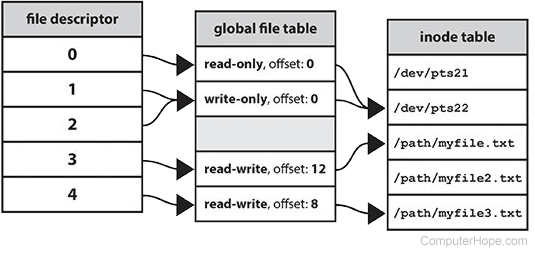
\includegraphics[width=0.5\textwidth]{figs/file_descriptor.png}
    \caption{قسمتی از فعالیت مربوط به \lr{file descriptor}}
    \label{fig:filedescriptor}
\end{figure}

\subsection{منظور از \lr{Task Control Block (TCB)}}

این بلاک در حقیقت وضعیت یک تسک را در سیستم عامل نگهداری می‌کند. این وضعیت شامل
مواردی مانند وضعیت فعلی فرایند، محل ذخیره‌سازی داده‌ها، شماره‌ی (اندیس) اطلاعات
زمانبندی، اطلاعات مربوط به حافظه مورد استفاده و شناسه تسک جاری است. رسالت اصلی
این اطلاعات آن است که به کرنل کمک کند تا تسک‌ها را از یکدیگر جدا نگه دارد. این
ساختار داده به عنوان یک پل بین کرنل و فرایند‌ها عمل می‌کند تا اطلاعات لازم را
برای کرنل جهت اداره منابع و برنامه‌ها را فراهم سازد.

\subsection{منظور از \lr{non-preemption}}

یکی از رویکرد‌های مهم در سیستم عامل‌های RT می‌باشد که از مفاهیم اولیه سیستم عامل
در زمانبندی انجام تسک‌ها آن را به یاد داریم. در کل به معنای آن است تا زمانی که
پردازنده در حال انجام یک تسک می‌باشد، تا زمانی که فعالیت پردازنده روی آن تسک به
پایان نرسیده باشد، پردازنده دیگری نمی‌تواند آن تسک را در اختیار بگیرد یا اینکه
برای مثلا پردازنده‌ای دیگر بخواهد برای مدت زمان مشخصی اجرای آن را متوقف یا به
طور کل قطع کند.

\section{سیستم مورد نظر این رویکرد}

\subsection{هدف اصلی}

هدف اصلی در سیستم عامل‌های Real-Time رسیدن به فرمول زیر به بهینه‌ترین حالت ممکن می‌باشد:

\begin{equation}
    t^{lim}_{ir} = t^{req}_{ir} - max(t_{fh}, t_{npl})
\end{equation}

\subsubsection{تعریف مولفه‌های مربوطه}

\begin{itemize}
    \item $t^{req}_{ir}$: مدت زمانی که طول می‌کشد تا به وقفه پیش آمده در
    رخداد‌های external مانند وقفه‌های تایمرها و وقفه‌های ورودی/خروجی پاسخدهی شود
    \item $t_{fh}$: مدت زمانی که طول می‌کشد تا \lr{fault hanlder} یک برنامه
    (Binary) به مشکل خورده را غیر فعال کند. تابع \lr{fault hanlder} در Thread
    های RT قابل کنترل هستند.
    \item $t_{npl}$: مدت زمانی که یک Thread در حال اجرا قفل غیر انحصاری را به
    دست می‌گیرد درست قبل از اینکه هر گونه وقفه‌ای رخ دهد.
\end{itemize}


هدف اصلی در این مقاله آن است که مدت زمان پاسخدهی بایستی از $t^{lim}_{ir}$ کوچکتر
و $t^{lim}_{ir} > 0$ باشد. بر اساس فرضیه، زمانی که Thread بخش RT مشغول است،
وقفه‌های بعدی در نظر گرفته نمی‌شوند. بعد از اینکه یک برنامه شکسته شده به طور
کامل متوقف شد، نیاز است که دوباره این برنامه به سرعت در چرخه اجرا قرار گیرد که
تقاضای ایجاد شده از بین نرود. دومین هدف در این رویکرد آن است که اجرای مجدد
برنامه شکسته شده در زمان $t^{req}_{re}$ بدون مزاحمت به thread های RT دیگر صورت
گیرد، شکل شماره \ref{fig:interruptHandlingDelayed}.

\subsection{محافظت از حافظه و سربار اجرایی}

اشتراک منابع بین تسک‌ها به صورت منطقی ممنوع است، اما تسک‌هایی مانند \lr{Message
Queue} و فرایند بین Pipeline ها که از دسته \lr{Intertask Communication} یا ITC
هستند می‌توانند از منابع یکدیگر استفاده کنند. از دلایلی که یک تسک می‌تواند به
صورت مدیریت شده به منابع تسک‌های دیگر دسترسی داشته باشد، آن است که واحد MPU
محافظت از حافظه در سیستم وجود نداشته باشد. در پردازنده‌های سری ARM Cortex-M/R،
یک واحد محافظت از حافظه MPU وجود دارد که ارتباط و دسترسی به حافظه فیزیکی را
براساس هر منطقه از حافظه انجام می‌دهد \cite{cortexm4arm}.

تعداد مناطقی که MPU اختصاص می‌دهد بین ۸ تا ۱۶ منطقه، متغیر می‌باشد. البته
می‌توان متذکر شد که این تعداد منطقه می‌تواند وابسته به پیکربندی مشتری بر روی
میکروکنترولر باشد. برای مثال، بعد از جست و جو مدل سری میکروکنترلر، به \lr{NXP
i.MX RT1020} رسیدیم که از ۱۶ منطقه دسترسی حافظه MPU استفاده می‌کند
\cite{armnxpimxrt1020}. در ادامه بررسی می‌کنیم که منطقه از MPU شامل چه بخش‌هایی
می‌باشد.

بخش‌های مهم حافظه MPU شامل موارد زیر است:

\begin{itemize}
    \item بخش آدرس
    \item بخش اندازه منطقه
    \item بخش ویژگی‌ها (برای مثال بررسی سطوح دسترسی)
\end{itemize}

بخش ویژگی‌ها یا Attributes مشخص می‌کنند که یک منطقه از حافظه توسط چه پردازنده‌ای
قابل استفاده برای تسک‌های مورد نظر خواهد بود. (بایستی در نظر داشت که هر منطقه از
MPU براساس ویژگی‌هایی مانند قابلیت اجرا Executable و Read-only بودن تنظیم و
پیکربندی می‌شود.) زمانی که یک پردازنده تلاش برای دسترسی به قسمتی از حافظه برای
نوشتن در آن می‌کند، MPU نوع دسترسی آن پردازنده را بررسی می‌کند و یک
\lr{Permission fault} تولید می‌کند \cite{armcortexm7} \cite{cortexm4arm}.

\begin{figure}
    \centering
    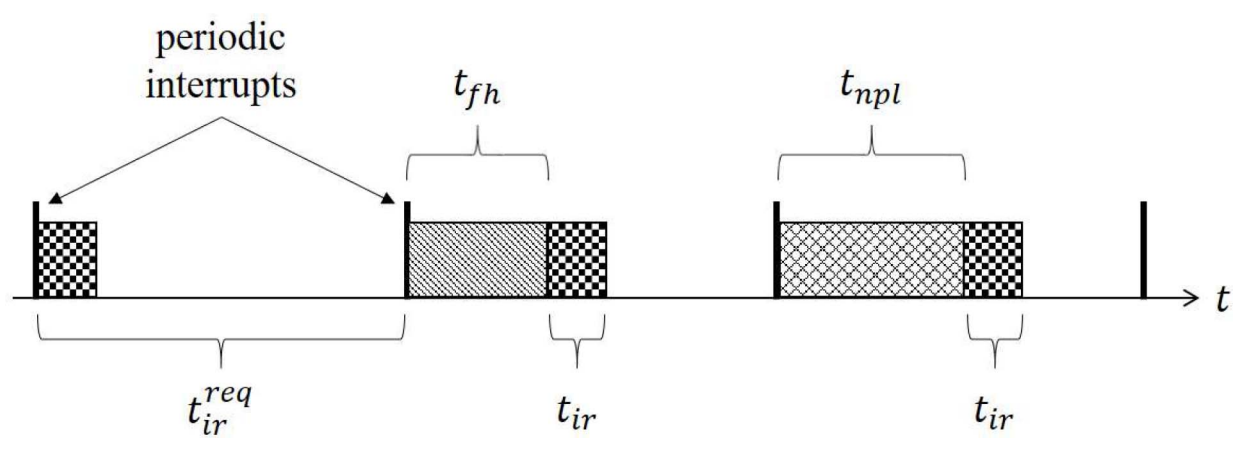
\includegraphics[width=0.5\textwidth]{figs/interrupt_handling_delay.png}
    \caption{دو مورد از وقفه‌هایی که رسیدگی به آن‌ها به تاخیر افتاده است}
    \label{fig:interruptHandlingDelayed}
\end{figure}

سیستم عامل TizenRT به عنوان یک سیستم‌عامل قابل اطمینان و پایدار IoT باید از سه
ناحیه MPU در RAM استفاده کند، هر کدام از ناحیه‌ها ویژگی‌های MPU متفاوتی برای
محافظت از یک برنامه کاربر دارد. متن و داده‌های Read-only تنها در ناحیه فقط
خواندنی MPU قرار می‌گیرد. داده‌های RW در ناحیه مناسب در حافظه کپی می‌شوند و
بخش‌هایی مانند استک و هیپ در حافظه‌ای مشابه ایجاد می‌شوند.

اگر بد‌افزاری قصد حمله به سیستم عامل از طریق ویرایش متن و دسترسی به دیتا، برای
اجرای برنامه خود داشته باشد، سیستم عامل از ورود آن جلوگیری کرده چرا که باعث آسیب
پذیری و رخ دادن خطای داخلی در سیستم عامل  می‌شود.  همانطور که قبل‌تر بیان شد،
Thread ها واحدی برای زمانبندی هستند به همین خاطر بعد از هر بار \lr{Context
Switching} بایستی سه ناحیه MPU به روز رسانی شود.

\subsubsection{نتیجه یک پروفایل و بنچمارک ساده با وجود محافظ و بدون وجود محافظ}

برای ارزیابی سربار حاصل شده با وجود حافظه MPU آزمایشی ساده صورت گرفته است. دو
Thread با بالاترین اولویت تنها یک تابع به نام \lr{sched\_yield()} را صدا
می‌زنند. تابع \lr{sched\_yield()} Thread جاری را از پردازنده می‌گیرد و آن را به
لیست آماده اجرای Thread ها بر می‌گرداند. در این بین باید توجه داشت که هیچ thread
فعال دیگری با همان اولویت در حال اجرا نیست.  بنابراین thread فراخوانده شده بعد
از thread دیگر قرار می‌گیرد که منجر به اصلاح زمان کمتری برای عملیات \lr{Context
switching} می‌شود. هر Thread تابع \lr{sched\_yield()} را $5.10^6$ بار صدا می‌زند
که مقدار $10^7$ بار عملیات \lr{Context switching} تکرار می‌شود. نتیجه این آزمایش
نشان می‌دهد که کمترین زمان عملیات \lr{Context switching} با وجود MPU $5.568\mu s$ و
بدون وجود MPU $5.466\mu s$ زمان می‌برد. می‌توان نتیجه گرفت که با وجود حافظه محافظ،
سربار ۱/۸۷٪ در عملیات \lr{Context switching} به وجود آمده است که این هزینه‌ی
اضافی برای محافظ حافظه اجتناب ناپذیر است اما از نظر اجرایی بسیار بی‌اهمیت
می‌باشد.

\subsection{راه‌اندازی آزمایشی}

در این آزمایش از محیط عملیاتی و سخت‌افزار زیر استفاده شده است:

\begin{enumerate}
    \item تمام عملیات سیستم عامل RT بر روی \lr{NXP i.MX RT1020}
    \cite{armnxpimxrt1020} صورت گرفته است.
    \item حاوی پردازنده ARM و چیپ سری Cortex-M7 با ۵۰۰ مگاهرتبز
    \item سخت افزاری مناسب برای دستگاه‌های هوشمند و سیستم کنترل کننده موتور در
    وسایل هوشمند خانگی
    \item یک حافظه SRAM با حجم ۲۵۶ کیلوبات
    \item حافظه خارجی با حجم ۳۲ مگابایت \lr{SDRAM (Synchronous Dynamic RAM)}
    \item سیستم عامل TizenRT نسخه ۳/۰ \cite{tizenrtrepo}
    \item کامپایل سیستم عامل با نسخه ۶/۳/۱ کامپایلر \lr{ARM GCC}
    \item استفاده در توزیع Ubuntu نسخه ۱۴/۰/۴
\end{enumerate}

\section{سیستم عامل قابل اطمینان و پایدار IoT}

از آنجایی که پایداری سیستم عامل برای تجهیزات IoT امری بسیار ضروری است، چرخه
فعالیت تمام برنامه‌های کاربر بایستی مدیریت و کنترل شوند. چرخه زندگی و فعالیت یک
برنامه کاربر می‌تواند اجرا در زمان بوت شدن باشد، یا اجرای مجدد آن برنامه به دلیل
آنکه خطایی یا شکست در برنامه‌ای رخ داده است باشد. این سیستم عامل بجای متوقف کردن
کل سیستم عامل به دلیل خطای رخ داده، آن برنامه‌ای که حاوی خطا است را پیدا می‌کند
و به مدیریت برنامه (\lr{Binary Manager}) اطلاع می‌دهد که چه برنامه‌ای هم اکنون
دچار شکست شده است. این امر امکان پذیر است چرا که محافظ حافظه تضمین می‌کند که
خطای رخ داده تنها در یک برنامه کاربر اتفاق افتاده است تا آن را از سیستم عامل جدا
کند که از سرایت خطا به بخش‌های دیگر جلوگیری نماید. مدیر برنامه درخواست‌های
متعددی را رسیدگی می‌کند. از واحد رسیدگی خطا و شکست برنامه گرفته تا را‌ه‌اندازی
اولیه سیستم عامل و حتی به روز رسانی برنامه کلاینت.

واحد مدیر برنامه می‌تواند حافظه heap برنامه کاربر را به صورت مناسب در زمان اجرا
\footnote{\lr{Runtime}} تنظیم کند. برای مثال زمانی که برنامه کاربر درخواست
افزایش حافظه heap را صادر می‌کند و بعد از آن در هنگام اجرا به خطای \lr{malloc()}
مواجه می‌شود واحد مدیر برنامه، برنامه به خطا خورده و حافظه کمکی‌اش را راه‌اندازی
مجدد می‌کند تا بتواند ادامه فرایند را طی کند. علاوه‌بر این زمانی که برنامه کاربر
حافظه حجیمی از heap را رزرو می‌کند ولی از آن به صورت مناسب استفاده نمی‌کند، واحد
مدیر برنامه قادر به آن است که این حافظه را از برنامه کاربر بگیرد تا باعث سربار
اضافی در سیستم نشود.


\bibliographystyle{elsarticle-num}
\bibliography{lib.bib}
\end{document}